\documentclass{beamer}

\usepackage{graphicx}
\usepackage{textpos}
\usepackage{listings}
\usepackage{tikz}
\usepackage{xcolor}
\usepackage{listofitems}

\definecolor{codegreen}{rgb}{0,0.6,0}
\definecolor{codegray}{rgb}{0.5,0.5,0.5}
\definecolor{codepurple}{rgb}{0.58,0,0.82}
\definecolor{backcolour}{rgb}{0.95,0.95,0.92}


\lstdefinestyle{py}{
  backgroundcolor=\color{backcolour},   
  commentstyle=\color{codegreen},
  keywordstyle=\color{magenta},
  numberstyle=\tiny\color{codegray},
  stringstyle=\color{codepurple},
  basicstyle=\ttfamily\footnotesize,
  breakatwhitespace=false,         
  breaklines=true,                 
  captionpos=b,                    
  keepspaces=true,                 
  numbers=left,                    
  numbersep=5pt,                  
  showspaces=false,                
  showstringspaces=false,
  showtabs=false,                  
  tabsize=2
}

\lstset{style=py}

\usetheme{Madrid}
\useoutertheme{miniframes} % Alternatively: miniframes, infolines, split

% Setup the university's color pallette
\definecolor{UIUCorange}{RGB}{19, 41, 75} 
\definecolor{UIUCblue}{RGB}{232, 74, 39} 


\setbeamercolor{palette primary}{bg=UIUCorange,fg=white}
\setbeamercolor{palette secondary}{bg=UIUCblue,fg=white}
\setbeamercolor{palette tertiary}{bg=UIUCblue,fg=white}
\setbeamercolor{palette quaternary}{bg=UIUCblue,fg=white}
\setbeamercolor{structure}{fg=UIUCorange} % itemize, enumerate, etc
\setbeamercolor{section in toc}{fg=UIUCblue} % TOC sections

\setbeamercolor{subsection in head/foot}{bg=UIUCorange,fg=UIUCblue}
\setbeamercolor{subsection in head/foot}{bg=UIUCorange,fg=UIUCblue}

\usepackage[utf8]{inputenc}
\usepackage{graphicx}

%Information to be included in the title page:
\title{\textbf{Topic 1: Programming, Spreadsheets, and Computers}}
\author{\textbf{David H Smith IV}}
\institute[\textbf{UIUC}]{\textbf{University of Illinois Urbana-Champaign}}
\date{\textbf{Wed, June 16 2021}}

\setbeamertemplate{title page}[default][colsep=-4bp,rounded=true]
\addtobeamertemplate{title page}{\vspace{3\baselineskip}}{}
\addtobeamertemplate{title page}{
  \begin{textblock*}{\paperwidth}(-1.0em, -1.2em)
    
\includegraphics[width=\paperwidth, height=\paperheight]{imgs/uiuc.png}
  \end{textblock*} 
}{}



\begin{document}

\frame{\titlepage}

\begin{frame}
  \frametitle{Updates}
  \begin{enumerate}
    \item zyBooks (participation activities) Topic 2 Assigned - Due Sunday at 11:00 PM CST
    \item Homework 1 - Due Friday at 11:00 PM CST
    \item Topic 1 zyBooks/Post-Reading 1 Extension - Due Sunday at 11:00 PM CST
    \item First quiz is next week:
      \begin{enumerate}
        \item First lab section (SDA) please login to the CBTF scheduler and register for the exam.
        \item Second lab section please check your email and reply to the messsge I sent yesterday.
      \end{enumerate}
  \end{enumerate}
\end{frame}

%
% 
%
\begin{frame}[fragile]
  \frametitle{Poll Question: Input and Print}
  Assuming there is a variable value with the value 7, which of the following statements prints: count = 7.
  \begin{enumerate}
    \item \lstinline{print("count = " value)}
    \item \lstinline{print("count = ", end="value")}
    \item \lstinline{print("count = ", value)}
    \item \lstinline{print("count = $value")}
  \end{enumerate}
\end{frame}

%
%
%
\begin{frame}
  \frametitle{Poll Question: Addition Operation}
  In Python x + y is:
  \begin{enumerate}
    \item an assignment
    \item a statement
    \item a variable
    \item an expression
    \item a comment
  \end{enumerate}
\end{frame}

%
%
%
\begin{frame}[fragile]
  \frametitle{Poll Question: Errors}
  What happens if I type the following code into a \textbf{brand new} Python interpreter:
  \begin{lstlisting}[language=Python]
  x + y \end{lstlisting}
  \begin{enumerate}
    \item Nothing
    \item SyntaxError
    \item NameError
    \item ValueError
    \item TypeError
  \end{enumerate}
\end{frame}

%
%
%
\begin{frame}[fragile]
  \frametitle{Poll Question: Error}
  What happens if I type the following code into a Python interpreter?
  \begin{lstlisting}[language=Python]
  print(input("Enter a number: "))\end{lstlisting}
  \begin{enumerate}
    \item No error
    \item SyntaxError
    \item NameError
    \item ValueError
    \item TypeError
  \end{enumerate}
\end{frame}

%
%
%
\begin{frame}[fragile]
  \frametitle{Poll Question: Errors}
  What happens if I type the following code into a Python interpreter?
  \begin{lstlisting}[language=Python]
  value = input("Input your favorite number!\n")
  print("Your new favorite number is", value + 1)\end{lstlisting}
  \begin{enumerate}
    \item No error
    \item SyntaxError
    \item NameError
    \item ValueError
    \item TypeError
  \end{enumerate}
\end{frame}

%
%
%
\begin{frame}[fragile]
  \frametitle{Poll Question: The Print Function}
  What type of error will Python produce when this segment of code is run?
  \begin{lstlisting}[language=Python]
  x = "Hello, world"
  y = 5
  foo = x + y + z\end{lstlisting}
  \begin{enumerate}
    \item SyntaxError
    \item NameError
    \item ValueError
    \item TypeError
  \end{enumerate}
\end{frame}

%
%
%
\begin{frame}[fragile]
  \frametitle{Poll Question: Data Types}
  What is the value of x after the following segment of code runs if the user inputs a 5 and then a 4?
  \begin{lstlisting}[language=Python]
  a = input()
  b = input()
  x = a + b\end{lstlisting}
  \begin{enumerate}
    \item String
    \item Integer
  \end{enumerate}
\end{frame}

%
%
%
\begin{frame}[fragile]
  \frametitle{Poll Question: Error}
  What happens if I type the following into a Python interpreter?
  \begin{lstlisting}[language=Python]
  a = input()
  b = input()
  a + b = x \end{lstlisting}
  \begin{enumerate}
    \item No error
    \item SyntaxError
    \item NameError
    \item ValueError
    \item TypeError
  \end{enumerate}
\end{frame}

%
%
%
%\begin{frame}[fragile]
%  \frametitle{Poll Question: Spreadsheets}
%  If I copy the contents of B1 to C4 what formula will be in C4?
%  \vfill
%  \begin{minipage}{.48\textwidth}
%    \begin{enumerate}
%      \item \lstinline{=$A0 + 2}
%      \item \lstinline{=$A2 + 2}
%      \item \lstinline{=$A3 + 2}
%      \item \lstinline{=$C0 + 2}
%      \item \lstinline{=$C2 + 2}
%      \item \lstinline{=$C3 + 2}
%    \end{enumerate}
%  \end{minipage}
%  \begin{minipage}{.48\textwidth}
%    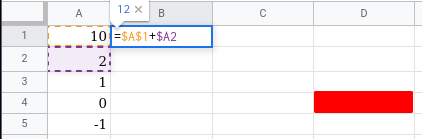
\includegraphics[width=\textwidth]{./imgs/spreadsheet-slide-2.png}
%  \end{minipage}
%\end{frame}

%
%
%
%\begin{frame}[fragile]
%  \frametitle{Poll Question: Spreadsheets}
%  What will be the expression when the cell at B0 is copied to D4?
%  \vfill
%  \begin{minipage}{.48\textwidth}
%    \begin{enumerate}
%      \item 
%    \end{enumerate}
%  \end{minipage}
%  \begin{minipage}{.48\textwidth}
%    \includegraphics[width=\textwidth]{./imgs/spreadsheet-slide-3.png}
%  \end{minipage}
%\end{frame}


%
%
%
\begin{frame}
  \frametitle{Your Questions!}
\end{frame}


\end{document}
